\message{ !name(background.tex)}
\message{ !name(background.tex) !offset(-2) }
\chapter{Background on Anomaly Detection through Scikit-Learn}

\section{What is Anomaly Detection?}
Anomaly Detection (AD in short, and depending of the application domain, outlier detection, novelty detection, deviation detection, exception mining) generally consists in assuming that the dataset under study contains a \textit{small} number of anomalies, generated by distribution models that  \textit{differ} from that generating the vast majority of the data.
 % anomalies are a \textit{small} number of observations generated by \textit{different} models from the one generating the rest of the data
%\sout{ -- the only difference in novelty detection is that the novel patterns are incorporated into the normal model after being detected. }.
This formulation motivates many statistical AD methods, based on the underlying assumption that anomalies occur in low probability regions of the data generating process. Here and hereafter, the term `normal data' does not refer to Gaussian distributed data, but  to  \emph{not abnormal} ones, \ie~data belonging to the above mentioned majority. 
Classical parametric techniques, like those developed in \cite{Barnett94} or in \cite{Eskin2000}, assume that the normal data are generated by a distribution belonging to some  specific, known in advance parametric model.  
The most popular non-parametric approaches include algorithms based on density (level set) estimation (see \textit{e.g.} \cite{Scholkopf2001},  \cite{Scott2006} or \cite{Breunig2000LOF}), on dimensionality reduction (\textit{cf} \cite{Shyu2003}, \cite{Aggarwal2001}) or on decision trees (\cite{Liu2008}).
% %approach is statistical, \
% % {\red donner le theme de chaque papier cité}
% \cite{Eskin2000},
% \cite{Desforges1998}, \cite{Barnett94}, \cite{Hawkins1980}
% , distance
% based, \cite{Knorr98}, \cite{Knorr2000}, \cite{Eskin2002geometric},
% local-density based \cite{Breunig2000LOF}, \cite{Breunig99LOF},
% \cite{Tang2002enhancing}, \cite{Papadimitriou2003loci}, spectral based
% \cite{Shyu2003}, \cite{Wang2006}, \cite{Lee2013} and others
% \cite{Aggarwal2001}, \cite{Kriegel2008}, \cite{Liu2008}. 
One may refer to \cite{Hodge2004survey}, \cite{Chandola2009survey}, \cite{Patcha2007survey} and \cite{Markou2003survey} for excellent overviews of current research on Anomaly Detection, ad-hoc techniques being far too numerous to be listed here in an exhaustive manner.


 Most usual AD algorithms actually
provide more than a predicted label for any new observation, abnormal vs. normal. Instead,
they return a real valued function,  termed a \textit{scoring function} sometimes, defining a preorder/ranking on the input space. Such a function permits to rank any observations according to their supposed `degree of abnormality' and thresholding it yields a decision rule that splits the input space into `normal' and `abnormal' regions.
In various fields (\textit{e.g.} fleet management, monitoring of energy/transportation networks), when confronted with massive data, being able to rank observations according to their degree of abnormality may significantly improve operational processes and allow for a prioritization of actions to be taken, especially in situations where human expertise required to check each observation is time-consuming.


From a machine learning perspective, AD can be considered as a specific classification task, where the usual assumption in supervised learning stipulating that the dataset contains structural information regarding all classes breaks down, see \cite{Roberts99}. This typically happens in the case of two highly unbalanced classes: the normal class is expected to regroup a large majority of the dataset, so that the very small number of points representing the abnormal class does not allow to learn information about this class.
In a clustering based approach, it can be
interpreted as the presence of a single cluster, corresponding to the
normal data. The abnormal ones are too limited to share a commun
structure, \ie~to form a second cluster. Their only characteristic is
precisely to lie outside the normal cluster, namely to lack any
structure.  Thus, common classification approaches may not be applied
as such, even in a supervised
context. % That is the reason why even in a supervised framework, common classification approaches cannot be applied.
\textbf{Supervised} AD consists in training the algorithm on a labeled (normal/abnormal) dataset including both normal and abnormal observations. In the \textbf{semi-supervised} context, only normal data are available for training. This is the case in applications where normal operations are known but intrusion/attacks/viruses are unknown and should be detected. In the \textbf{unsupervised} setup, no assumption is made on the data which consist in unlabeled normal and abnormal instances. In general, a method from the semi-supervised framework may apply to the unsupervised one, as soon as the number of anomalies is sufficiently weak to prevent the algorithm from fitting them when learning the normal behavior. Such a method should be robust to outlying observations.


Contribution of this thesis includes the implemention of two classical AD algorithms on the open-source Scikit-Learn library (\cite{sklearn2011}), namely the Isolation Forest algorithm (\cite{Liu2008}) and the Local Outlier Factor algorithm (\cite{Breunig2000LOF}).
The following section provides insights on Anomaly Detection through Scikit-Learn by describing and comparing AD algorithms from this library. Part of this section are modified versions of the documentation included in the forementioned scikit-learn contribution.

\section{Anomaly Detection in Scikit-learn}
\label{sec:AD_sklearn}

\subsection{What is Scikit-learn?}
Scikit-learn, see \cite{sklearn2011}, is an open-source library which provides well-established machine learning methods.
It is a Python module, the latter language being a very popular for scientific computing, thanks to its high-level interactive nature. Python is enjoying this recent years a strong expansion both in academic and industrial settings. Scikit-learn takes advantage of this favourable backdrop and extends this general-purpose programming language with machine learning operation: it not only provides implementations of many established algorithms, both supervised and unsupervised, while keeping an easy-to-use interface tightly integrated with the Python language. It also provides a composition mechanism (through a \emph{Pipeline} object) to combine estimators, preprocessing tools and model selection methods in such a way the user can easily constructs complex ad-hoc algorithms.

Scikit-Learn depends only on \emph{numpy} (the base data structure used for data and model parameters, see \cite{Vanderwalt2011numpy}) and \emph{scipy} (to handle common numerical operations, see \cite{Jones2015scipy}).
Most of the Scikit-learn package is written in python and \emph{cython}, a compiled programming language for combining C in Python to achieve the performance of C with high-level programming in Python-like syntax.


The development is done on \emph{github}\footnote{https://github.com/scikit-learn}, a Git repository hosting service which facilitates collaboration, as coding is done in strong interaction with other developpers. Because of the large number of developers, emphasis is put on keeping the project maintainable, \eg~by avoiding dupplicating code up to pay (reasonably) in computational performance. As an example, the initial Isolation Forest implementation contained a complementary cython code to efficiently browse the trees of the forest. This functionality was included in an other (more complete) tree browser, but which is heavier in terms of computation. A balance had to be made between the computational gain and the maintainability cost, which led to choose the last one.


Scikit-learn benefits from a simple and consistent API (Application Programming Interface), see \cite{sklearn_api2013}, through the \emph{estimator} interface. This interface is followed by all (supervised and unsupervised) learning algorithms as well as other tasks such as preprocessing ones, feature extraction and selection. The central object \emph{estimator} implements a \emph{fit} method to learn from training data, taking as argument an input data array (and optionnally an array of labels for supervised problems). The initialization of the estimator is done separately, before training, in such a way the constructor don't see any data and can be seen as a function taking as input the model hyper-parameters and returning the learning algorithm initialized with this parameters. Relevant default parameters are provided for each algorithm. To illustrate initialization and fit steps, the snippet below consider an anomaly detection learning task with the \emph{Isolation Forest} algorithm.

\begin{pythoncode} 
# Import the IsolationForest algorithm from the ensemble module
from sklearn.ensemble import IsolationForest
# Instantiate with specified hyper-parameters
IF = IsolationForest(n_trees=100, max_samples=256)
# Fit the model on training data (build the trees of the forest)
IF.fit(X_train)
\end{pythoncode}
%
In this code example, the Isolation Forest algorithm is imported from the \emph{ensemble} module of Scikit-learn, which contains the ensemble-based estimators such as bagging or boosting methods. Then, an \tsf{IsolationForest} instance \tsf{IF} is initialized with a number of trees of $100$ (see Section~\ref{sec:iforest} for details on this algorithm). Finally, the model is learned from training data \tsf{X\_train} and stored on the \tsf{IF} object for later use. Since all estimators share the same API, it is possible to train a Local Outlier Factor algorithm by simply replacing the constructor name \tsf{IsolationForest(n\_trees=100)} in the snippet above by \tsf{LocalOutlierFactor()}.

Some estimators (such as supervised estimators or some of the unsupervised ones, like Isolation Forest and LOF algorithm) are called \emph{predictors} and implement a \emph{predict} method that takes a data array and returns predictions (labels or values computed by the model). Other estimators (\eg~PCA) are called \emph{transformer} and implement a \emph{transform} method returning modified input data.
The following code example illustrates how simple it is to predict labels with the predictor interface. It suffices to add the line of code below to the previous snippet.
\begin{pythoncode} 
# Perform prediction on new data
y_pred = IF.predict(X_test)  
# Here y_pred is a vector of binary labels (+1 if inlier, -1 if abnormal)
\end{pythoncode}



%\chapter{A performance criterion: the Mass-Volume Curve}

%\subsection{Elliptic Envelop}

\subsection{One-class SVM}

The SVM algorithm is essentially a two-class algorithm (\ie~one needs negative as well as positive examples).
\cite{Scholkopf2001} extended the SVM methodology to handle training using only positive information:
the One-Class Support Vector Machine (OCSVM) treats the origin as the only member of the second class (after mapping the data to some feature space). Thus the OCSVM finds a separating hyperplane between the origin and the mapped one class, using some `relaxation parameters'.

The OCSVM consists in estimating Minimum Volume (MV) sets, which amounts (if the density has no flat parts) to estimating density level sets, as mentionned in the introduction.
%
% As a good sketch is better than a long speech, we refer to 
Figures~\ref{table:OCSVM-hard} and \ref{table:OCSVM-hard}  summarizes the theoretical insights of OCSVM compared to the standard SVM, respectively for the hard-margin (no error is tolerated during training) and soft-margin separation (some margin errors are tolerated in training).
\renewcommand{\arraystretch}{2.5}
\begin{table}[h!]
  \centering
  \begin{tabular}{|c|c|}\hline
    SVM                                                             &    OCSVM  \\ \hline 
    $\displaystyle \min_{w,b} \frac{1}{2} \|w\|^2$                   & $\displaystyle \min_{w} \frac{1}{2} \|w\|^2$   \\
    s.t~~~~ $\forall i,~~y_i(\langle w, x_i\rangle + b) \ge 1$      & s.t~~~~ $\forall i,~~\langle w, x_i\rangle ~\ge 1$ \\ \cdashline{1-2}
    \multicolumn{2}{|l|}{~}\\
    \multicolumn{2}{|l|}{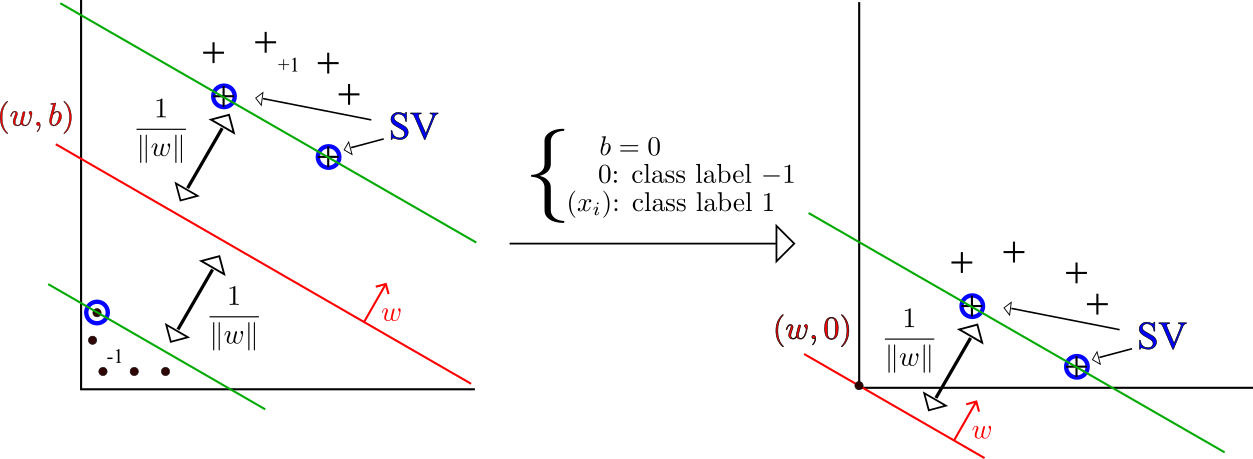
\includegraphics[scale=0.83]{fig_source/OCSVM_hard}} \\\cdashline{1-2}
    decision function:                                             & decision function:  \\
    ~~~~~~~~$f(x) = \text{sgn}(\langle w, x\rangle + b)$ ({\red red line}) ~~~~~~~ & $f(x) = \text{sgn}(\langle w, x\rangle - 1)$ ({\green green line}) \\ \cdashline{1-2} 
    \multicolumn{2}{|l|}{-Lagrange multipliers: $\alpha_i$ ~~~~($\alpha_i>0$ when the constraint is an equality for $x_i$)} \\
    \multicolumn{2}{|l|}{-Support vectors: $\text{SV} = \{ x_i,~~ \alpha_i > 0\}$ }\\
    \multicolumn{2}{|l|}{-Margin errors: $\text{ME} = \emptyset $ ~~~~~~~~~~~~~~~ }\\ \cdashline{1-2}
    $\displaystyle w = \sum_i \alpha_i y_i x_i$                    & $\displaystyle w = \sum_i \alpha_i x_i$  \\ \hline 
  \end{tabular}
  \caption{SVM vs. OCSVM (hard-margin separation)}
  \label{table:OCSVM-hard}
\end{table}

\begin{table}[h!]
  \centering
  \begin{tabular}{|c|c|}\hline
    SVM                                                             &    OCSVM  \\ \hline 
    $\displaystyle \min_{w,\xi,\rho,b} \frac{1}{2} \|w\|^2 + \frac{1}{n} \sum_{i=1}^n \xi_i - \nu \rho$ & $\displaystyle \min_{w,\xi,\rho} \frac{1}{2} \|w\|^2 + \frac{1}{n} \sum_{i=1}^n \xi_i - \nu \rho$  \\
    s.t~~~~ $\forall i, ~~y_i(\langle w, x_i\rangle ~+~ b) \ge \rho - \xi_i$                        & s.t~~~~ $\forall i,~~\langle w, x_i\rangle ~\ge \rho - \xi_i $ ~~~~~~\\ 
    $\xi_i \ge 0$ ~~~~~~~~~~~~~~~~~~~~~                                                            & $\xi_i \ge 0$~~~~~~~~~~~~  \\ \cdashline{1-2}
    \multicolumn{2}{|l|}{~}\\
    \multicolumn{2}{|l|}{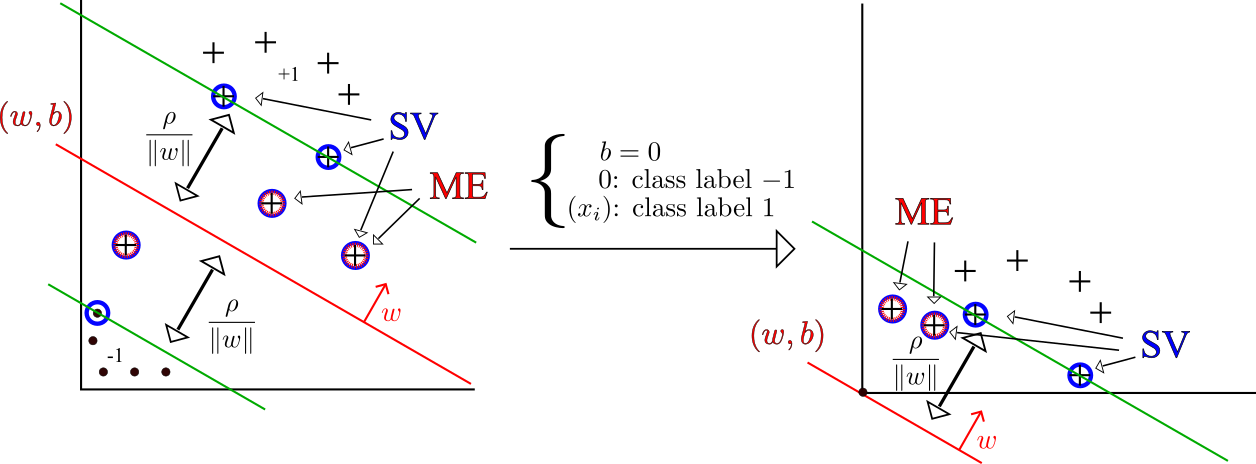
\includegraphics[scale=0.83]{fig_source/OCSVM_soft}} \\\cdashline{1-2}
    decision function:                                                                             & decision function:  \\
    ~~~~~~~~$f(x) = \text{sgn}(\langle w, x\rangle + b)$ ({\red red line}) ~~~~~~~            & $f(x) = \text{sgn}(\langle w, x\rangle - \rho)$ ({\green green line})\\ \cdashline{1-2}
    \multicolumn{2}{|l|}{-Lagrange multipliers: $\alpha_i, \beta_i$ ~~~~(one for each constraint, $\beta_i > 0$ when $\xi_i = 0$)}\\
    \multicolumn{2}{|l|}{-Support vectors: $\text{SV} = \{ x_i,~~ \alpha_i > 0\}$ }\\
    \multicolumn{2}{|l|}{-Margin errors: $\text{ME} = \{x_i,~~ \xi_i > 0 \} =  \{x_i,~~ \beta_i > 0 \} $ ~~~(for OCSVM, ME=anomalies) }\\
    \multicolumn{2}{|l|}{-$\text{SV} \setminus \text{ME} = \{ x_i,~~ \alpha_i, \beta_i > 0\}$ }\\ \cdashline{1-2}
    $w = \sum_i \alpha_i y_i x_i$                                                                   & $w = \sum_i \alpha_i x_i$  \\ \cdashline{1-2}
    \multicolumn{2}{|c|}{ $\displaystyle \frac{|\text{ME}|}{n} ~\le~ \nu ~\le~ \frac{|\text{SV}|}{n}$ }   \\
    \multicolumn{2}{|c|}{$\displaystyle \rho = \langle w, x_i\rangle ~~~~\forall x_i \in \text{SV} \setminus \text{ME}$} \\ \hline

              
  \end{tabular}
  \caption{SVM vs. OCSVM ($\nu$-soft margin separation)}
  \label{table:OCSVM-soft}
\end{table}

In the $\nu$-soft margin separation framework, letting $\Phi$ be the mapping function determined by a kernel function $k$ (\ie~$k(x,y) = \langle \Phi(x), \Phi(y)\rangle$), the separating hyperplan defined \wrt~a vector $w$ and an offset $\rho$ is given by the solution of 
\begin{align*}
&\min_{w,\xi,\rho} \frac{1}{2} \|w\|^2 + \frac{1}{n} \sum_{i=1}^n \xi_i - \nu \rho\\
&\text{s.t.}~~~ \langle w, \Phi(x_i)\rangle ~\ge \rho - \xi_i~~,~~~~~~1 \le i \le n \\
& ~~~~~~~~\xi_i \ge 0,
\end{align*}
where $\nu$ is previously fixed. An interesting fact is that $\nu$ is an upper bound on the fraction of outliers and a lower bound on the fraction of support vectors, both of which converging to $\nu$ almost surely when $n \to \infty$ (under some continuity assumption). Then, the empirical mass of the estimated level set is greater than $1-\nu$ and converges almost surely to $1-\nu$ as $n$ tends to infinity. Hence one usual approach is to choose $\nu = 1 - \alpha$ to estimate a MV-set with mass (at least) $\alpha$. For insights on the calibration of One-Class SVM, see for instance \cite{Thomas2015}.
%
The complexity of OCSVM training is the same as for the standard SVM, namely $O(n^3 d)$ where $n$ is the number of samples and $d$ the dimension of the input space. However, one can expect a complexity of $O(n^2 d)$, see \cite{Bottou2007}. From its linear complexity \wrt~the number of features $d$, OCSVM scales well in large dimension, and performance remains good even when the dimension is greater than $n$. By using only a small subset of the training dataset (support vectors) in the decision function, it is memory efficient. However, OCSVM suffers from practical limitation: 1) the non-linear training complexity in the number of observations, which limits its use on very large datasets; 2) its sensitivity to the parameter $\nu$ and to the kernel parameter, which makes callibration tricky; 3)
parametrization of the mass of the MV set estimated by the OCSVM via the parameter $\nu$ does not allow to obtain nested set estimates as the mass $\alpha$ increases.  

\subsection{Local Outlier Factor algorithm}
One other very efficient way of performing outlier detection in datasets whose dimension is moderately large is to use the Local Outlier Factor (LOF) algorithm proposed in \cite{Breunig2000LOF}.

This algorithm computes a score reflecting the degree of abnormality of the observations, the so-called local outlier factor. It measures the local deviation of a given data point with respect to its neighbors. By comparing the local density near a sample to the local densities of its neighbors, one can identify points which have a substantially lower density than their neighbors. These are considered to be outliers.

In practice the local density is obtained from the $k$-nearest neighbors. The LOF score of an observation is equal to the ratio of the average local density of his $k$-nearest neighbors, and his own local density: a normal instance is expected to have a local density similar to that of its neighbors, while abnormal data are expected to have much smaller local density.

The strength of the LOF algorithm is that it takes both local and global properties of datasets into consideration: it can perform well even in datasets where abnormal samples have different underlying densities. The question is not, how isolated the sample is, but how isolated it is with respect to the surrounding neighborhood.

This strategy is illustrated in the code example below, returning Figure~\ref{fig:lof}.
\begin{figure}[!h]
  %\centering
  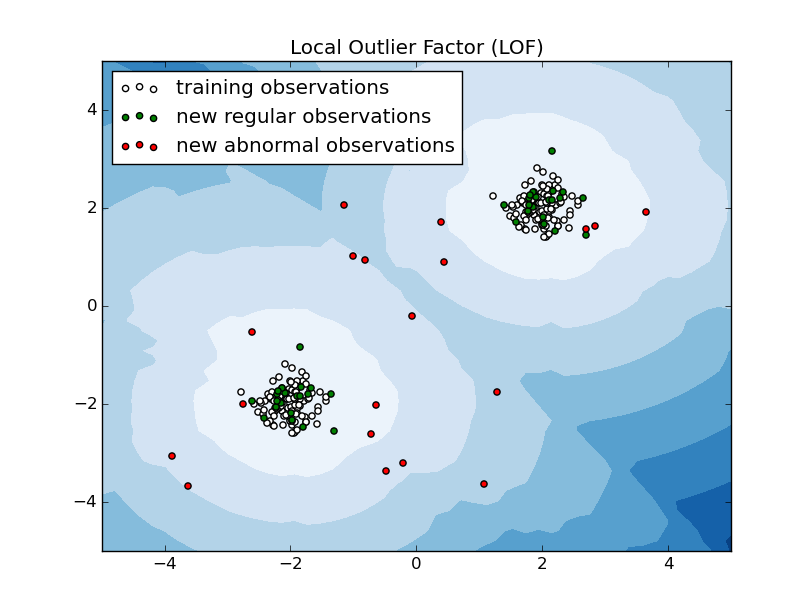
\includegraphics[width=0.9\linewidth]{fig_source/lof}
  \caption{LOF example}
  \label{fig:lof}
\end{figure}

\begin{pythoncode} 
"""
=================================================
Anomaly detection with Local Outlier Factor (LOF)
=================================================

This example uses the LocalOutlierFactor estimator
for anomaly detection.
"""

import numpy as np
import matplotlib.pyplot as plt
from sklearn.neighbors import LocalOutlierFactor

np.random.seed(42)

# Generate train data
X = 0.3 * np.random.randn(100, 2)
X_train = np.r_[X + 2, X - 2]
# Generate some regular novel observations
X = 0.3 * np.random.randn(20, 2)
X_test = np.r_[X + 2, X - 2]
# Generate some abnormal novel observations
X_outliers = np.random.uniform(low=-4, high=4, size=(20, 2))

# fit the model
clf = LocalOutlierFactor()
clf.fit(X_train)
y_pred_train = clf.predict(X_train)
y_pred_test = clf.predict(X_test)
y_pred_outliers = clf.predict(X_outliers)

# plot the line, the samples, and the nearest vectors to the plane
xx, yy = np.meshgrid(np.linspace(-5, 5, 50), np.linspace(-5, 5, 50))
Z = clf.decision_function(np.c_[xx.ravel(), yy.ravel()])
Z = Z.reshape(xx.shape)

plt.title("Local Outlier Factor (LOF)")
plt.contourf(xx, yy, Z, cmap=plt.cm.Blues_r)

b1 = plt.scatter(X_train[:, 0], X_train[:, 1], c='white')
b2 = plt.scatter(X_test[:, 0], X_test[:, 1], c='green')
c = plt.scatter(X_outliers[:, 0], X_outliers[:, 1], c='red')
plt.axis('tight')
plt.xlim((-5, 5))
plt.ylim((-5, 5))
plt.legend([b1, b2, c],
           ["training observations",
            "new regular observations", "new abnormal observations"],
           loc="upper left")
plt.show()
\end{pythoncode}




\subsection{Isolation Forest}
\label{sec:iforest}


One efficient way of performing outlier detection in high-dimensional datasets
is to use random forests.
%
The IsolationForest proposed in \cite{Liu2008} 'isolates' observations by randomly selecting a feature and then randomly selecting a split value between the maximum and minimum values of the selected feature.
%
Since recursive partitioning can be represented by a tree structure, the
number of splittings required to isolate a sample is equivalent to the path
length from the root node to the terminating node.
%
This path length, averaged over a forest of such random trees, is a measure
of abnormality and our decision function.
%
Random partitioning produces noticeable shorter paths for anomalies, see Figure~\ref{fig:ideeIF}. Moreover, the average depth of a sample over the forest seems to converge to some limits, the latter being different depending on if the sample is or not an anomaly.
Hence, when a forest of random trees collectively produce shorter path lengths
for particular samples, they are highly likely to be anomalies.
%
This strategy is illustrated in the code example below returning Figure~\ref{fig:iforest}.


\begin{minipage}{0.52\linewidth}
\centering
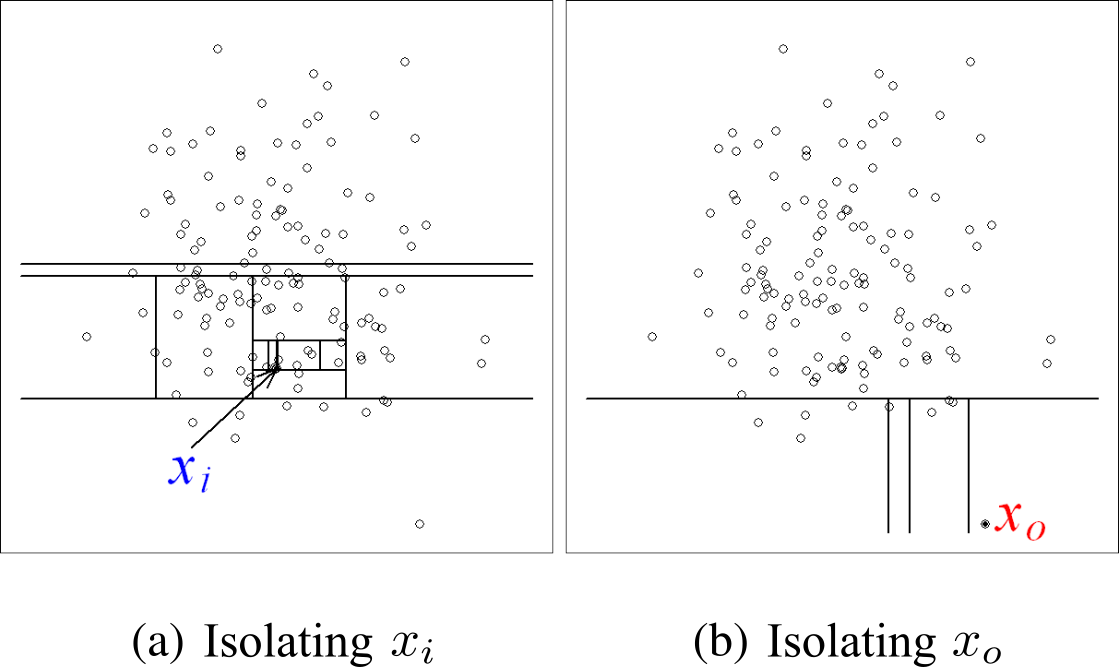
\includegraphics[scale=.95]{fig_source/ideeIF}
\captionof{figure}{Anomalies are isolated more quickly}
\label{fig:ideeIF}
\end{minipage}\hfill
\begin{minipage}{0.52\linewidth}
\centering
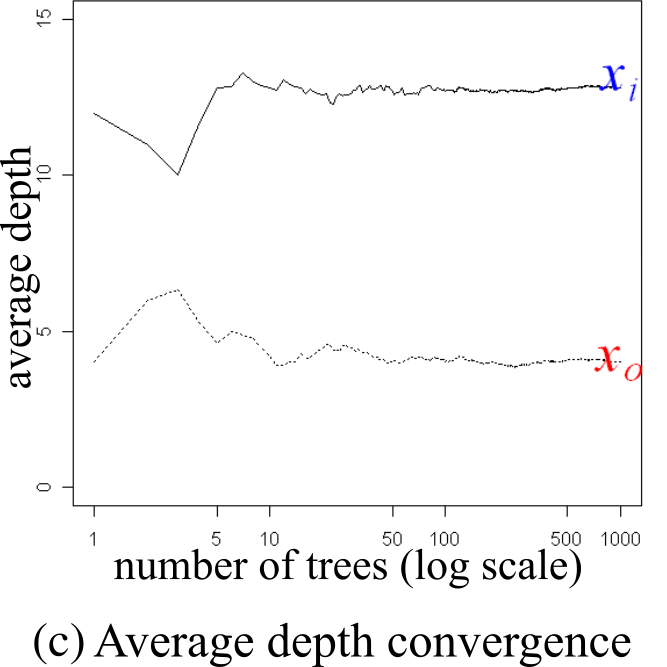
\includegraphics[scale=.95]{fig_source/convergenceIF}
\captionof{figure}{Convergence of the averaged depth}
\label{2Dcones}
\end{minipage}


\begin{figure}[!h]
\centering
  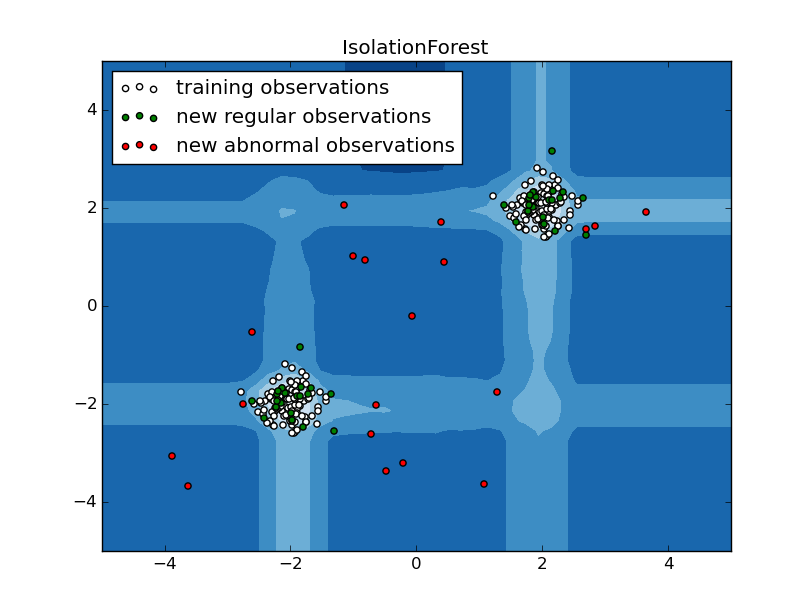
\includegraphics[width=0.8\linewidth]{fig_source/iforest}
  \caption{Isolation Forest example}
  \label{fig:iforest}
\end{figure}
~\\
\begin{pythoncode} 
"""
==========================================
IsolationForest example
==========================================

An example using IsolationForest for anomaly detection.

"""

import numpy as np
import matplotlib.pyplot as plt
from sklearn.ensemble import IsolationForest

rng = np.random.RandomState(42)

# Generate train data
X = 0.3 * rng.randn(100, 2)
X_train = np.r_[X + 2, X - 2]
# Generate some regular novel observations
X = 0.3 * rng.randn(20, 2)
X_test = np.r_[X + 2, X - 2]
# Generate some abnormal novel observations
X_outliers = rng.uniform(low=-4, high=4, size=(20, 2))

# fit the model
clf = IsolationForest(max_samples=100, random_state=rng)
clf.fit(X_train)
y_pred_train = clf.predict(X_train)
y_pred_test = clf.predict(X_test)
y_pred_outliers = clf.predict(X_outliers)

# plot the line, the samples, and the nearest vectors to the plane
xx, yy = np.meshgrid(np.linspace(-5, 5, 50), np.linspace(-5, 5, 50))
Z = clf.decision_function(np.c_[xx.ravel(), yy.ravel()])
Z = Z.reshape(xx.shape)

plt.title("IsolationForest")
plt.contourf(xx, yy, Z, cmap=plt.cm.Blues_r)

b1 = plt.scatter(X_train[:, 0], X_train[:, 1], c='white')
b2 = plt.scatter(X_test[:, 0], X_test[:, 1], c='green')
c = plt.scatter(X_outliers[:, 0], X_outliers[:, 1], c='red')
plt.axis('tight')
plt.xlim((-5, 5))
plt.ylim((-5, 5))
plt.legend([b1, b2, c],
           ["training observations",
            "new regular observations", "new abnormal observations"],
           loc="upper left")
plt.show()
\end{pythoncode}

As a conclusion of this Section,
Figures~\ref{fig:ADcomparison1}, \ref{fig:ADcomparison2} and \ref{fig:ADcomparison3} draw a comparison of the three anomaly detection algorithm introduced in this section:

- the One-Class SVM which is able to capture the shape of the
  data set, hence performing well when the data is strongly
  non-Gaussian, i.e. with two well-separated clusters;

- the Isolation Forest algorithm, which is adapted to
  large-dimensional settings, even if it performs quite well in the
  examples below.

- the Local Outlier Factor which measures the local deviation of a given
  data point with respect to its neighbors by comparing their local density.

The ground truth about inliers and outliers is given by the points colors
while the orange-filled area indicates which points are reported as inliers
by each method.

Here, we assume that we know the fraction of outliers in the datasets.
Thus rather than using the 'predict' method of the objects, we set the
threshold on the decision function to separate out the corresponding
fraction. Anomalies are uniformly drawn according to an uniform distribution.


\begin{figure}[H]
  \centering
  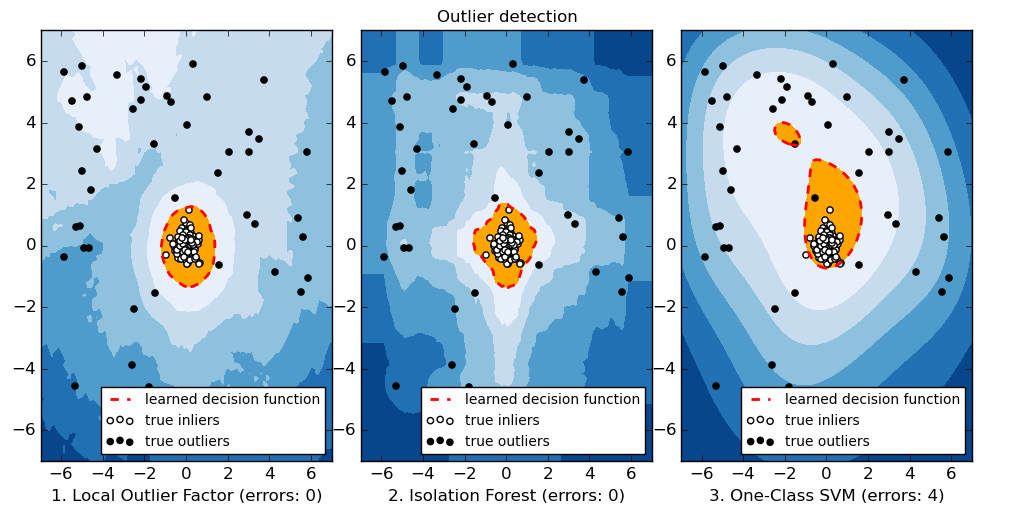
\includegraphics[width=.9\linewidth]{fig_source/ADcomparison1}
  \caption{gaussian normal data with one single mode}
  \label{fig:ADcomparison1}
\end{figure}

\begin{figure}[H]
  \centering
  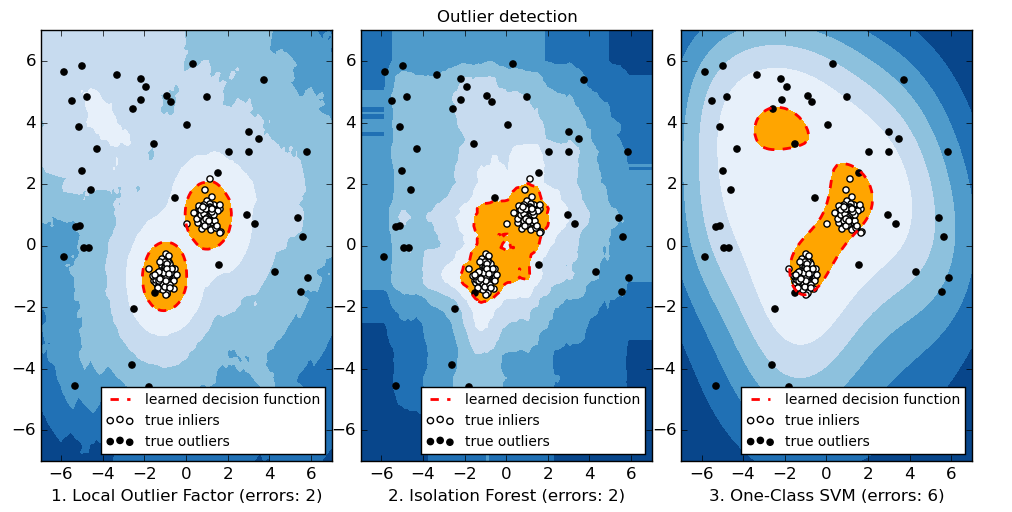
\includegraphics[width=.9\linewidth]{fig_source/ADcomparison2}
  \caption{gaussian normal data with two modes}
  \label{fig:ADcomparison2}
\end{figure}

\begin{figure}[H]
  \centering
  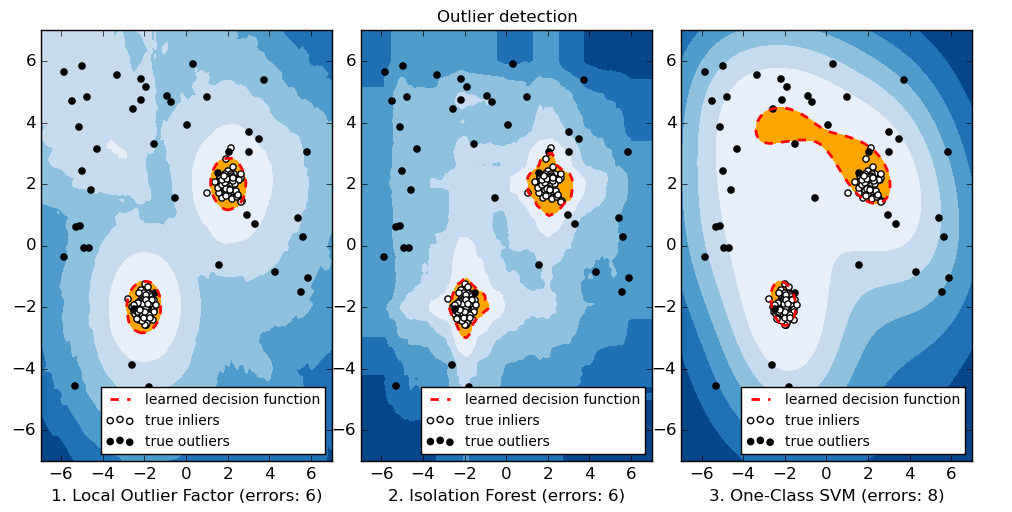
\includegraphics[width=.9\linewidth]{fig_source/ADcomparison3}
  \caption{gaussian normal data with two strongly separate modes}
  \label{fig:ADcomparison3}
\end{figure}

% as the following code is longer than 1 page, bgcolor=lightgray option does not work: we have to use mdframed package
\begin{mdframed}[hidealllines=true, backgroundcolor=lightgray] 
\begin{minted}[fontfamily=courier, fontsize=\scriptsize]{python}
"""
==========================================
Outlier detection with several methods.
==========================================
"""

import numpy as np
import matplotlib.pyplot as plt
import matplotlib.font_manager
from scipy import stats

from sklearn import svm
from sklearn.covariance import EllipticEnvelope
from sklearn.ensemble import IsolationForest
from sklearn.neighbors import LocalOutlierFactor

rng = np.random.RandomState(42)

# Example settings
n_samples = 200
outliers_fraction = 0.25
clusters_separation = [0, 1, 2]

# define two outlier detection tools to be compared
classifiers = {
    "One-Class SVM": svm.OneClassSVM(nu=0.95 * outliers_fraction + 0.05,
                                     kernel="rbf", gamma=0.1),
    #"robust covariance estimator": EllipticEnvelope(contamination=.25),
    "Isolation Forest": IsolationForest(random_state=rng),
    "Local Outlier Factor": LocalOutlierFactor(n_neighbors=35, contamination=0.25)}

# Compare given classifiers under given settings
xx, yy = np.meshgrid(np.linspace(-7, 7, 100), np.linspace(-7, 7, 100))
n_inliers = int((1. - outliers_fraction) * n_samples)
n_outliers = int(outliers_fraction * n_samples)
ground_truth = np.ones(n_samples, dtype=int)
ground_truth[-n_outliers:] = 0

# Fit the problem with varying cluster separation
for i, offset in enumerate(clusters_separation):
    np.random.seed(42)
    # Data generation
    X1 = 0.3 * np.random.randn(n_inliers // 2, 2) - offset
    X2 = 0.3 * np.random.randn(n_inliers // 2, 2) + offset
    X = np.r_[X1, X2]
    # Add outliers
    X = np.r_[X, np.random.uniform(low=-6, high=6, size=(n_outliers, 2))]

    # Fit the model
    plt.figure(figsize=(10, 5))
    for i, (clf_name, clf) in enumerate(classifiers.items()):
        # fit the data and tag outliers
        clf.fit(X)
        y_pred = clf.decision_function(X).ravel()
        threshold = stats.scoreatpercentile(y_pred,
                                            100 * outliers_fraction)
        y_pred = y_pred > threshold
        n_errors = (y_pred != ground_truth).sum()
        # plot the levels lines and the points
        Z = clf.decision_function(np.c_[xx.ravel(), yy.ravel()])
        Z = Z.reshape(xx.shape)
        subplot = plt.subplot(1, 3, i + 1)
        subplot.contourf(xx, yy, Z, levels=np.linspace(Z.min(), threshold, 7),
                         cmap=plt.cm.Blues_r)
        a = subplot.contour(xx, yy, Z, levels=[threshold],
                            linewidths=2, colors='red')
        subplot.contourf(xx, yy, Z, levels=[threshold, Z.max()],
                         colors='orange')
        b = subplot.scatter(X[:-n_outliers, 0], X[:-n_outliers, 1], c='white')
        c = subplot.scatter(X[-n_outliers:, 0], X[-n_outliers:, 1], c='black')
        subplot.axis('tight')
        subplot.legend(
            [a.collections[0], b, c],
            ['learned decision function', 'true inliers', 'true outliers'],
            prop=matplotlib.font_manager.FontProperties(size=10),
            loc='lower right')
        subplot.set_xlabel("%d. %s (errors: %d)" % (i + 1, clf_name, n_errors))
        subplot.set_xlim((-7, 7))
        subplot.set_ylim((-7, 7))
    plt.subplots_adjust(0.04, 0.1, 0.96, 0.94, 0.1, 0.26)
    plt.suptitle("Outlier detection")

plt.show()
\end{minted}
\end{mdframed}

\chapter{Concentration Inequalities from the Method of bounded differences}
% XXXX TODO: add memoire + CONCENTRATION

This chapter presents general results on measure concentration inequalities, obtained via a martingal method, the method of bounded differences. We recommend \cite{McDiarmid98} and \cite{Janson2002} for good references on this subject, and \cite{BLM2013} for an complete review on concentration inequalities.
%  Ce document présente des résultats généraux sur les inégalités de concentration de mesure et quelques applications, notamment aux graphes aléatoires.
% Il est basé sur les articles de Colin McDiarmid "Concentration", de Terence Tao "Talagrand's concentration inequality", et de Svante Janson "On concentration of probability".
% Dans ce travail, j'ai choisi de mettre en relation les trois articles de la facon suivante : J'utilise l'article de McDiarmid pour illustrer et démontrer dans un cadre plus général les résultats fondamentaux exposés dans l'article de Janson, dont le but est de donner un survol des différentes méthodes pour obtenir des inégalités de concentration. J'ai choisi quelques applications présentées par McDiarmid, ainsi que dans l'article de Tao.
%Nous verrons deux méthodes pour obtenir des inégalités de concentration : la méthode des différences bornées, qui est une méthode de martingales, puis la méthode assez récente due à Talagrand, qui donne souvent des résultats plus forts que la précédente.



\section{Two fundamental results}
The two following results allow to derive lots of classical concentration inequalities, like
Hoeffding, Azuma, Bernstein or McDiarmid inequalities.

\subsection{Preliminary definitions}
Let $(\Omega,\mathcal{F},\mathbb{P})$ be a probability space.
Let $X$ be a random variable on this space and $\mathcal{G}$ a sub-$\sigma$-algebra of $\mathcal{F}$.

\begin{definition} Assume $X$ is a real \rv. We then define $\sup(X|\mathcal{G})$ as the unique real \rv~$f:\Omega \rightarrow \mathbb{R}$ verifying:
\begin{itemize}
\item[(i)] $f$ is $\mathcal{G}$-measurable
\item[(ii)] $X \leq f$ a.s.
\item[(iii)] If  $g:\Omega \rightarrow \mathbb{R}$ verifies (i) and (ii) then $ f\le g$ a.s.
\end{itemize}
\end{definition}

Note that we clearly have $\sup(X|\mathcal{G}) \geq \mathbb{E}(X|\mathcal{G}) $ and  $\sup(X|\mathcal{G}_1) \geq  \sup(X|\mathcal{G}_2) $ when  $ \mathcal{G}_1 \subset \mathcal{G}_2$ .


\begin{definition}
\label{defpreli1}
Assume $X$ is bounded. Let $(\mathcal{F}_k)_{0\leq k \leq n}$ be a filtration of $\mathcal{F}$ such that $X$ is $\mathcal{F}_n$-mesurable. We denote $X_1,...,X_n$ the martingale $X_k=\mathbb{E}(X|\mathcal{F}_k)$ and $Y_k=X_k - X_{k-1}$ the associated martingale difference. The \rv~$\mathbf{ran(X \vert \mathcal{G})} := \sup(X | \mathcal{G}) + \sup(-X \vert \mathcal{G}) $ is called the conditional range of $X$ \wrt~ $\mathcal{G}$. Then we define:
\begin{itemize}
\item [$\star$] $ \mathbf{ran_k} = ran (Y_k|\mathcal{F}_{k-1}) = ran(X_k|\mathcal{F}_{k-1})$ the conditional range,
\item [$\star$] $\mathbf{R^2} = \sum_{1}^{n} ran_k^2$  the sum of squared conditional ranges, and $\mathbf{\hat{r}^2} = \supess(R^2)$ the maximum sum of squared conditional ranges.
\end{itemize}
\end{definition}

\begin{definition}
We place ourselves in the same context as the previous definition, but without assuming $X$ bounded. The \rv~$\mathbf{var(X|\mathcal{G})} := \mathbb{E}((X-\mathbb{E}(X|\mathcal{G}))^2|\mathcal{G}) $ is called the conditional variance of $X$ \wrt~$\mathcal{G}$. Then we define:
\begin{itemize}
\item [$\bullet$] $\mathbf{var_k} = var(Y_k|\mathcal{F}_{k-1})=var(X_k|\mathcal{F}_{k-1})$ the conditional variance, 
\item [$\bullet$] $\mathbf{V} = \sum_{1}^{n} var_k$ the sum of conditional variances and $\hat\nu= \supess(V)$ the maximum sum of conditional variances,
\item [$\ast$] $\mathbf{dev_k^+} = \sup(Y_k|\mathcal{F}_{k-1})$ the conditional positive deviation,
\item  [$\ast$] $\mathbf{maxdev^+} $ = $ \supess(\displaystyle\max_{0 \leq k \leq n}~ dev_k^+)$  the maximum conditional positive deviation.
\end{itemize}
\end{definition}

The \rv~$V$ is also called the `predictable quadratic variation' of the martingale $(X_k)$ and verifies $\mathbb{E}(V)= var(X)$.


\subsection{Statements}

\begin{theorem}
\label{3.14}
Let $X$ a bounded \rv~with $\mathbb{E}(X)=\mu$, and $(\mathcal{F}_k)_{0\leq k \leq n}$ a filtration of $\mathcal{F}$ such that $ \mathcal{F}_0 =  (\emptyset , \Omega) $ and such that $X$ is $\mathcal{F}_n$-measurable. 
Then for any $t \geq 0$, $$\mathbb{P}(X-\mu \geq t) \leq e^{-2t^2/\hat r^2},$$ and more generally $$\forall r^2 \geq 0,~~~ \mathbb{P}((X-\mu \geq t)\cap(R^2 \leq r^2)) \leq e^{-2t^2/ r^2}.$$
\end{theorem}

To prove this result we need the two following lemmas.
On a besoin des deux lemmes suivants, qui sont faciles à prouver (le premier par récurrence, le second en utilisant la convexité de $x \rightarrow e^{hx}$:


\begin{lemma}
 \label{lemme_mg}
Soit $(\mathcal{F}_k)_{0\leq k \leq n}$ une filtration de $\mathcal{F}$ avec $ \mathcal{F}_0 =  (\emptyset , \Omega) $. Soit $(Y_k)_{1 \leq k \leq n}$ une différence de martingale pour cette filtration telle que chaque $Y_k$ soit borné. Soit Z une fonction indicatrice. Alors :
\begin{eqnarray*} \mathbb{E}(Z e^{h\sum Y_k}) \leq \sup(Z \prod_{k} \mathbb{E}(e^{hY_k}|\mathcal{F}_{k-1} ))
\end{eqnarray*}
\end{lemma}
\begin{proof}
This result can be easily proved by induction:


\end{proof}
\begin{remark} Ce lemme joue en quelque sorte le même role que l'indépendance des termes d'une somme de variables, si on oublie le "sup".
\end{remark}

\begin{lemma} 
 \label{lemme_u}
Soit X une variable aléatoire telle que $\mathbb{E}(X) = 0 $ et $a \leq X \leq b$, alors $ \forall h>0, \mathbb{E}(e^{hX}) \leq e^{\frac{1}{8}h^2(b-a)^2} $.
Ce résultat reste vrai avec des espérances conditionnelles (la condition est alors $ \mathbb{E}(X|\mathcal{G})=0$) .
\end{lemma}

\begin{proof} (théorème \ref{3.14}) :

La preuve du théorème (\ref{3.14}) suit un schéma "traditionnel", comme on le verra dans la preuve directe de l'inégalité d'Hoeffding, basée en trois étapes : L'inégalité de Markov exponentielle, la majoration du terme exponentielle par indépendance (ou dans le cas présent par le lemme utile (\ref{lemme_mg}), qui joue le même rôle), puis par le lemme utile (\ref{lemme_u}). Enfin l'optimisation en $h$ : 

Soit $X_k=\mathbb{E}(X|\mathcal{F}_{k-1})$ et $Y_k=X_k-X_{k-1}$ la différence de martingales associée.
On pose $  Z=\mathds{1}_{R^2 \leq r^2}  $. \\
L'inégalité de Markov exponentielle donne,
 \begin{eqnarray*} \forall h, ~
\mathbb{P}((X-\mu \geq t)\cap(R^2 \leq r^2)) 
 &=& \mathbb{P}(Ze^{h(X-\mu)} \geq e^{ht})\\
 &\leq& e^{-ht}\mathbb{E}(Ze^{h(X-\mu)})\\
 &\leq& e^{-ht}\mathbb{E}(Ze^{h(\sum Y_k)}) 
 \end{eqnarray*}
\\ 

Par le lemme utile (\ref{lemme_u}), 
$ \mathbb{E}(e^{hY_k}|\mathcal{F}_{k-1}) \leq e^{\frac{1}{8}h^2r_k^2}$ \\
D'où par le lemme utile (\ref{lemme_mg})  :
\begin{eqnarray*}
 \mathbb{E}(Ze^{h\sum Y_k}) &\leq& \sup(Z \prod \mathbb{E}(e^{hY_k}|\mathcal{F}_{k-1}))\\
& \leq & \sup(Z \prod e^{\frac{1}{8}h^2 r_k^2})\\
&=&  \sup(Z e^{\frac{1}{8}h^2R^2})\\
&\leq& e^{\frac{1}{8}\sup(ZR^2)}\\
&\leq& e^{\frac{1}{8}h^2r^2}
\end{eqnarray*}

Finalement, on obtient :
 \begin{eqnarray*}
 \mathbb{P}((X-\mu \geq t)\cap(R^2 \leq r^2)) \leq e^{-ht+\frac{1}{8}h^2r^2} \leq e^{-2t^2/r^2}
 \end{eqnarray*} 
en posant $h=\frac{4t}{r^2}$.

\end{proof}

\begin{theorem}
\label{3.15}
Soit X une variable aléatoire avec $\mathbb{E}(X)=\mu$ et $(\mathcal{F}_k)_{0\leq k \leq n}$ une filtration de $\mathcal{F}$ avec $ \mathcal{F}_0 =  (\emptyset , \Omega) $ et telle que X est $\mathcal{F}_n$-mesurable.
Soit $b=maxdev^+$ la déviation conditionnelle maximale supposée finie, et $\hat\nu=\supess V$ la somme maximale des variances conditionnelles supposée finie également. \\
Alors $\forall t \geq 0,~ \mathbb{P}(X-\mu \geq t) \leq e^{-\frac{t^2}{2(\hat\nu+bt/3)}}$\\
et plus généralement $\forall t \geq 0, \forall v \geq 0,~ \mathbb{P}((X-\mu \geq t)\cap(V \leq v)) \leq e^{-\frac{t^2}{2(v+bt/3)}}$.

\end{theorem}

Nous avons besoin de deux lemmes : le lemme utile (\ref{lemme_mg}) ci-dessus exploitant la décomposition en somme de différences de martingales et remplacant l'indépendance des termes de cette somme dans la preuve, et le lemme suivant qui joue le même rôle que le lemme utile (\ref{lemme_u}) pour des variables non necessairement bornées mais à variance bornée :

\begin{lemma}
\label{lemme_u2}
Soit g la fonction croissante définie par $\forall x \neq 0,~ g(x)=\frac{e^x-1-x}{x^2}$, et X une variable aléatoire satisfaisant $\mathbb{E}(X)=0$ et $X \leq b$. \\
Alors $\mathbb{E}(X) \leq e^{g(b)var(X)}$.
Ce résultat reste vrai avec des espérances et des variances conditionnelles en remplacant $b$ par $\sup(X|\mathcal{G})$.
\end{lemma}
La preuve de ce lemme est immédiate en remarquant que $e^x \leq 1+x+x^2g(b)$ pour $x \leq b$.

\begin{proof} (théorème (\ref{3.15})) :
Elle suit le même schéma classique que le théorème (\ref{3.14}).
Soient $Y_1,...,Y_n$ les différences de martingales associées à $X$ et à $(\mathcal{F}_k)$ .

On pose $  Z=\mathds{1}_{V \leq v}  $. \\
L'inégalité de Markov exponentielle donne,
 \begin{eqnarray*} \forall h, ~
\mathbb{P}((X-\mu \geq t)\cap(V \leq v)) 
 &=& \mathbb{P}(Ze^{h(X-\mu)} \geq e^{ht})\\
 &\leq& e^{-ht}\mathbb{E}(Ze^{h(X-\mu)})\\
 &\leq& e^{-ht}\mathbb{E}(Ze^{h(\sum Y_k)}) 
 \end{eqnarray*}
\\ 

Par le lemme utile (\ref{lemme_u2}), 
$ \mathbb{E}(e^{hY_k}|\mathcal{F}_{k-1}) \leq e^{h^2g(hdev_k^+)var_k} \leq e^{h^2g(hb)var_k} $ \\
D'où par le lemme utile (\ref{lemme_mg}) :
\begin{eqnarray*}
 \mathbb{E}(Ze^{h\sum Y_k}) &\leq& \sup(Z \prod \mathbb{E}(e^{hY_k}|\mathcal{F}_{k-1}))\\
& \leq & \sup(Z \prod e^{h^2g(hb)var_k})\\
&=&  \sup(Z e^{h^2g(hb)V})\\
&\leq& e^{h^2g(hb)\sup(ZV)}\\
&\leq& e^{h^2g(hb)v}
\end{eqnarray*}


Finalement, on obtient :

\begin{eqnarray*} \mathbb{P}((X-\mu \geq t)\cap(R^2 \leq r^2)) &\leq& e^{-ht+h^2g(hb)v}\\
&\leq&  e^{-\frac{t^2}{2(v+bt/3)}}
\end{eqnarray*}

en posant $h=\frac{1}{b}ln(1+\frac{bt}{v})$ puis en utilisant que $\forall x \geq 0,~ (1+x)ln(1+x)-x \geq 3x^2/(6+2x)$.

\end{proof}


\section{Inégalités célèbres}

\subsection{Sans hypothèse de variance}

\begin{theorem} (Inégalité de Azuma-Hoeffding)
\label{HA3.10}
Soit $(\mathcal{F}_k)_{0\leq k \leq n}$ une filtration de $\mathcal{F}$ avec $ \mathcal{F}_0 =  (\emptyset , \Omega) $, soit Z une martingale et Y la différence de martingale associée.
Si $\forall k, ~ |Y_{k}| \leq c_{k}$, alors :

$ \mathbb{P}(|\sum Y_k| \geq t) \leq 2 e^{-\frac{t^2}{2 \sum c_k^2}}$
 
\end{theorem}

\begin{proof}
On veut appliquer le théorème (\ref{3.14}) en posant $X=\sum_{1}^{n}Y_k$, $\mathcal{F}_k=\sigma(Y_1,...,Y_k)$ et $X_k=\mathbb{E}(X|\mathcal{F}_k)$ :
On a alors $\mu=0$, $X_k=\mathbb{E}(X|\mathcal{F}_k)=\sum_{1}^{k}Y_i $ car Z martingale, et $Y_i=X_i-X_{i-1}$.\\
Donc $ran_k=ran(Y_k|\mathcal{F}_k) \leq 2c_k$ d'où $R^2 \leq 4 \sum c_k^2$ et $\hat r^2 \leq 4 \sum c_k^2$.\\
Par le théorème \ref{3.14}~~ $\mathbb{P}(X-\mu \geq t) \leq e^{\frac{-2t^2}{\hat r^2}} \leq e^{-\frac{t^2}{2\sum c_k^2}}$\\
En appliquant cette inégalité à -X, on obtient $ \mathbb{P}(|\sum Y_k| \geq t) \leq 2 e^{-\frac{t^2}{2 \sum c_k^2}}$.
\end{proof}

\begin{theorem} (Inégalité de McDiarmid)
\label{mcdiarmid}
Soit $X=(X_1,...,X_n)$ où les $X_i$ sont indépendants à valeurs dans $A_i$.
Soit $f : \prod A_k \rightarrow \mathbb{R}$ vérifiant la condition de Lipschitz:
\begin{eqnarray}
\forall x,x' \in \prod_{1}^{n} A_k,~ |f(x)-f(x')| \leq c_k ~~
\mbox{si x et x' ne diffèrent seulement de la kième coordonnée.}
\label{CL}
\end{eqnarray} 
On note $\mu=\mathbb{E}(f(X))$.
Alors $\forall t \geq 0, ~ \mathbb{P}(f(X)-\mu \geq t) \leq e^{-2t^2/\sum c_k^2}$\\ et donc $\forall t \geq 0, ~ \mathbb{P}(|f(X)-\mu| \geq t) \leq 2e^{-2t^2/\sum c_k^2}$
\end{theorem}


\begin{proof} La condition de Lipschitz (\ref{CL}) implique que $f$ est bornée, donc par le thèorème (\ref{3.14}) on a :\\
$\mathbb{P}(f(X)-\mu \geq t) \leq e^{-2t^2/\hat r^2}$ où $\hat r^2$ est défini en posant $\mathcal{F}_k=\sigma(X_1,...,X_k)$ et $X=f(X_1,...,X_n)$\\
On remarque que cette inégalité est vraie sans hypothèse d'indépendance ni de la condition de Lipschitz, seulement avec l'hypothèse f bornée. L'hypothèse de Lipschitz et l'indépendance vont permettent de majorer $\hat r^2$:\\
$ran_k=ran(~\mathbb{E}(f(X)|\mathcal{F}_k)-\mathbb{E}(f(X)|\mathcal{F}_{k-1})~~|\mathcal{F}_{k-1}) \leq c_k$

\end{proof}


\begin{theorem} (Inégalité de Hoeffding)
Soient $X_1,...,X_n$ variables indépendantes telles que $\forall i, ~ a_i \leq X_i \leq b_i$. Soit $S_n=\sum X_k$ et $\mu=\mathbb{E}(S_n)$.\\
Alors $\mathbb{P}(|S_n-\mu| \geq t) \leq 2e^{-2t^2/\sum(b_k-a_k)^2} $.
\end{theorem}

\begin{proof}
 Il s'agit d'une conséquence de l'inégalité de McDiarmid avec $ A_k=[a_k,b_k]$, $f(x)=\sum x_k$ et $c_k=b_k-a_k $. On a alors $\hat r^2 \leq b_k-a_k$.
\end{proof}

\begin{remark} 
 La preuve directe de ce résultat suit le même schéma que celle du théorème (\ref{3.14}): Inégalité de Markov exponentielle, puis hypothèse de somme de variables indépendantes (ou de différences de martingales), et enfin utilisation du lemme utile (\ref{lemme_u}) avant l'optimisation en h:
\begin{eqnarray*} 
\mathbb{P}(S_n-\mu \geq t) &\leq& \mathbb{E}(e^{h(S_n-\mu)})e^{-ht}\\
\mathbb{E}(\prod e^{h(X_k-\mathbb{E}X_k)})&=&\prod \mathbb{E}(e^{h(X_k-\mathbb{E}X_k)})\mbox{~par indépendance}\\
&\leq& e^{\frac{1}{8}h^2\sum(b_k-a_k)^2} \mbox{~par le lemme utile (\ref{lemme_u})}
\end{eqnarray*}
puis on pose $h=\frac{4t}{\sum(b_k-a_k)^2}$.
\end{remark}

\begin{remark} 
 On se rend compte en comparant ces deux dernières inégalités au théorème (\ref{3.14}) que la décomposition en somme de différences de martingales permet une généralisation du cas d'une somme de variables indépendantes. Sous réserve d'introduire des outils de contrôle plus précis comme $\hat r^2$, on n'a plus besoin d'indépendance ni de condition de Lipschitz.\\
Ces deux hypothèses supplémentaires peuvent être vues comme une manière de majorer $\hat r^2$ pour obtenir une forme plus simple.
\end{remark}

\subsection{Variance bornée}

\begin{theorem} (Bernstein)
\label{Bernstein}
Soient $X_1,...,X_n$ des variables aléatoires indépendantes avec $X_k-\mathbb{E}(X_k) \leq b$. On pose $S_n=\sum X_k$, $V=var(S_n)$ et $\mathbb{E}(S_n)=\mu$.
\begin{eqnarray*}
\mbox{Alors :~~~~~~~~~~~~~~~~}
\forall t \geq 0,~ \mathbb{P}(S_n-\mu \geq t) \leq e^{-\frac{t^2}{2(V+bt/3)}}\\
\mbox{et plus généralement :}~~~~ \mathbb{P}((S_n-\mu \geq t)\cap(V \leq v)) \leq e^{-\frac{t^2}{2(v+bt/3)}} 
\end{eqnarray*} 
\end{theorem}
\begin{proof}
On pose $F_k=\sigma(X_1,...,X_n)$ , $X=\sum (X_k-\mathbb{E}X_k) =S_n-\mu$ , $\tilde X_k=\mathbb{E}(X|\mathcal{F}_k)=\sum_{1}^{k}(X_i-\mathbb{E}X_i)$ et $Y_k=\tilde X_k - \tilde X_{k-1}$.\\
Alors~ $Y_k= X_k-\mathbb{E}X_k$ 
d'où~  $dev_k^+ \leq b$ puis $maxdev^+ \leq b $~ 
et $var_k=var(Y_k|\mathcal{F}_{k-1})=\mathbb{E}((Y_k-\mathbb{E}(Y_k|\mathcal{F}_{k-1}))^2|\mathcal{F}_{k-1})=\mathbb{E}((Y_k-\mathbb{E}Y_k)^2)=var(Y_k)$
donc $\hat \nu = \supess(\sum var_k)=\supess(V)=V$.\\
Le théorème (\ref{3.15}) s'applique donc et donne :
\begin{eqnarray*}
\mathbb{P}(S_n-\mu \geq t) \leq e^{-\frac{t^2}{2(V+bt/3)}}\\
\mathbb{P}((S_n-\mu \geq t)\cap(V \leq v)) \leq e^{-\frac{t^2}{2(v+bt/3)}}
\end{eqnarray*}
 
\end{proof}

\begin{theorem}
\label{3.12}
Soit $(Y_k)_{1 \leq k \leq n}$ une différence de martingale telle que $-a_k \leq Y_k \leq 1-a_k$, $a=\frac{1}{n} \sum a_k$ 
\begin{itemize}
\item[(i)] $\forall t \geq 0,~\mathbb{P}(|\sum Y_k| \geq t) \leq 2e^{-2t^2/n}$  
\item[(ii)] $\forall \epsilon > 0,~ \mathbb{P}(\sum Y_k \geq \epsilon an) \leq e^{-\frac{\epsilon^2an}{2(1+\epsilon / 3)}}$
\item[(iii)] $\forall \epsilon > 0,~ \mathbb{P}(\sum Y_k \leq -\epsilon an) \leq e^{-\frac{1}{2}\epsilon ^2 an}$
\end{itemize}

\end{theorem}

\begin{proof}
(i) est une conséquence immédiate du théorème (\ref{3.14}), puisque :  $-a_k \leq Y_k \leq 1-a_k ~~\Rightarrow~~ ran_k \leq 1 ~~\Rightarrow~~ \hat r^2 \leq n$\\\\
(ii) On pose $X=Z_n$, $\mathcal{F}_k=\sigma(Z_1,...,Z_k)$ et $\forall 1 \leq k \leq n, X_k = \mathbb{E}(X|\mathcal{F}_k)$.
On a $X_k=Z_k$ car $Z_k$ martingale, donc $Y_k=X_k-X_{k-1}$.\\
Comme $-a_k \leq Y_k \leq 1-a_k$, on a $dev_k^+=\sup(Y_k|\mathcal{F}_{k-1}) \leq 1$ et donc $b=maxdev^+ \leq 1$. \\
Soit $W_k:=Y_k+a_k$. On a $0\leq W_k \leq 1$, $\mathbb{E}(W_k|\mathcal{F}_{k-1})=a_k$ et $var(Y_k|\mathcal{F}_{k-1})=var(W_k|\mathcal{F}_{k-1})$.
Or :\begin{eqnarray*}
var(W_k|\mathcal{F}_{k-1})&=&\mathbb{E}(W_k^2|\mathcal{F}_{k-1})-\mathbb{E}(W_k|\mathcal{F}_{k-1})^2\\ &\leq& \mathbb{E}(W_k|\mathcal{F}_{k-1})-\mathbb{E}(W_k|\mathcal{F}_{k-1})^2\\&=&a_k-a_k^2\\&=&a_k(1-a_k)\\ &\leq& a_k 
\end{eqnarray*}
Donc $V=\sum var_k \leq \sum a_k = na$
 d'où $\hat \nu \leq na$\\
Le théorème (\ref{3.15}) donne donc :
\begin{eqnarray*}
\mathbb{P}(Z_n-Z_0 \geq t) \leq e^{-\frac{t^2}{2(\hat \nu + bt/3)}} \leq e^{-\frac{t^2}{2(an+t/3)}}\\
\mbox{d'où il suit que :  }~~~~ \mathbb{P}(\sum Y_k \geq \epsilon an) \leq e^{-\frac{\epsilon^2a^2n^2}{2(an+\epsilon an/3)}}= e^{-\frac{\epsilon^2an}{2(1+\epsilon/3)}}
\end{eqnarray*}

(iii) On a $-a_k\leq Y_k\leq 1-a_k ~~\Rightarrow~~ -\bar a_k \leq -Y_k \leq 1- \bar a_k $  où  $\bar a_k=1-a_k$.\\
En posant $\bar a = 1-a$, (ii) appliqué à $(-Y_k, \bar a_k)$ donne : 
 \begin{eqnarray*}
\forall \epsilon > 0,~ \mathbb{P}(\sum(-Y_k) \geq \epsilon \bar a n) \leq e^{-\frac{\epsilon ^2 \bar a n}{2(1+\epsilon/3)}}. 
\end{eqnarray*}
Avec $\epsilon = ta/\bar a$ on obtient :
\begin{eqnarray*}
\forall t > 0,~\mathbb{P}(\sum(-Y_k) \geq t a n) \leq e^{-\frac{t ^2  a n}{2(a \bar a+a^2t/3)}} 
\end{eqnarray*}
Comme $-Y_k \leq a_k$ on a $\sum(-Y_k) \leq an~ p.s.$~~   donc :
\begin{eqnarray}
\label{etoile} 
\forall t >1,~ \mathbb{P}(\sum(-Y_k) \geq tan)=0
\end{eqnarray}
De plus :   ~~~~$\forall t \in ]0,1],~ 2(a \bar a + a^2t/3) \leq 2(1/4 + 1/3) \leq 2$\\
\\Donc :
\begin{eqnarray*} 
\forall t \in ]0,1],~ \mathbb{P}(\sum(-Y_k) \geq tan) \leq e^{-\frac{1}{2}t^2an}
\end{eqnarray*}
ce qui est aussi valable pour $t>1$ par (\ref{etoile}).
Ainsi,  
\begin{eqnarray*}
\forall t > 0,~ \mathbb{P}(-\sum Y_k \geq tan) &\leq& e^{-\frac{1}{2}t^2an}\\
 \forall t > 0,~ \mathbb{P}(\sum Y_k \leq -tan) &\leq& e^{-\frac{1}{2}t^2an}
\end{eqnarray*}

\end{proof}


On déduit immédiatement de ce théorème (avec $a_k=\mathbb{E}(X_k)$, $Y_k=X_k-a_k$, ce qui donne $-a_k \leq Y_k \leq 1-a_k$ et $\sum Y_k= S_n - \mu$) le théorème bien connu suivant :

\begin{theorem}
Soient $X_1,...,X_n$ variables aléatoires indépendantes avec $0 \leq X_k \leq 1$ , $S_n= \sum X_k$,  $\mu=\mathbb{E} S_n$ et $p=\mu /n$. Alors :
\begin{itemize}
\item[(i)] $\forall  t > 0,~\mathbb{P}(S_n \geq \mu + t) \leq e^{-\frac{t^2}{2(\mu + t/3)}}$  
\item[(ii)] $\forall t > 0,~ \mathbb{P}(S_n \leq \mu-t) \leq e^{-\frac{t^2}{2 \mu}}$
\end{itemize}
\end{theorem} 

\section{Applications de la méthode des différences bornées au nombre chromatique}
Soit $G_{n,p}$ un graphe aléatoire à n sommets, tel que pour chaque pairs de ces sommets, il existe une arête les reliant avec probabilité $p$.
On note $E(G_{n,p})$ l'ensemble des arêtes de $G_{n,p}$.
Soit $(A_1,...,A_m)$ une partition de l'ensemble des arêtes possibles (i.e de l'ensemble des arêtes du graphe complet $\mathbb{K}_n$).
Alors $E(G_{n,p})$ peut s'écrire $(E_1,...,E_m)$ avec $E_i \in \mathcal{P}(A_i)$ et on identifie par la suite un graphe sur les $n$ sommets avec l'ensemble de ses arêtes qui s'écrit de manière unique dans $\prod_{1}^{m} \mathcal{P}(A_i)$.

\begin{theorem}
\label{3.2}
Soit $f$ une fonction sur l'ensemble des graphes sur les $n$ sommets telle que
\begin{eqnarray}
\label{4}
\exists k,~ E(G)\Delta E(G') \subset A_k ~~\Rightarrow~~ |f(G)-f(G')|\leq 1 
\end{eqnarray}
Alors la variable $Y:=f(G_{n,p})$ vérifie :
\begin{eqnarray*}
\forall t>0,~\mathbb{P}(Y-\mathbb{E}Y \geq t) \leq e^{-2t^2/m} \\
\end{eqnarray*}

\end{theorem}

\begin{proof}
Il s'agit de l'inégalité de McDiarmid (\ref{mcdiarmid}) appliquée à $X=E(G_{n,p})=(E_1,...,E_m) \in \prod_{1}^{m}\mathcal{P}(A_i)$ avec  $\forall 0 \leq k \leq m,~ c_k=1$.\\
En effet, la condition (\ref{4}) signifie simplement que si $E(G)$ et $E(G')$ ne diffèrent que de la kième coordonnée, alors $|f(G)-f(G')| \leq c_k = 1$.
\end{proof}


%\begin{corollary}
%\label{3.3}
%Supposons que $|f(G)-f(G')| \leq 1$ dès que $G'$ peut être obtenu à partir de $G$ en ne changeant que les arêtes reliées à un sommet fixé.
%Alors :
%\begin{eqnarray*}
%\forall t > 0,~ \mathbb{P}(f(G_{n,p})-\mathbb{E}f(G_{n,p}) \geq t) \leq e^{-2t^2/n}\\ 
%\end{eqnarray*}
%\end{corollary}

%\begin{proof} Il s'agit du théorème précédent (\ref{3.2}) appliqué avec $m=n$ et% $A_k=\{(j,k),j<k\}$ 
%\end{proof}

%On remarque que le nombre chromatique $\chi(G)$ vérifie la condition du corollai%re (\ref{3.3}). (Dans le pire des cas, on crée une couleur pour le sommet concer%né et $|\chi(G)-\chi(G')|\leq 1$)
%Donc : 
%\begin{eqnarray*}
%\mathbb{P}(|\chi(G)-\mathbb{E}(\chi(G))| \geq t) \leq 2e^{-2t^2/n} 
%\end{eqnarray*}

\begin{corollary}
\label{3.4}
Supposons que $|f(G)-f(G')| \leq 1$ dès que $G$ et $G'$ ne diffèrent que d'une arête.
Alors :
\begin{eqnarray*}
\forall t > 0, \mathbb{P}(f(G_{n,p})-\mathbb{E}f(G_{n,p}) \geq t) \leq e^{-4t^2/n^2} 
\end{eqnarray*} 
\end{corollary}

\begin{proof}
Il s'agit du théorème (\ref{3.2}) appliqué avec $m=\left( \begin{array}{c} n \\ 2
\end{array} \right)$ et $\forall i, |A_i|=1$ :
\begin{eqnarray*}
 \forall t > 0, \mathbb{P}(f(G_{n,p})-\mathbb{E} G_{n,p} \geq t) \leq e^{-\frac{2t^2}{n(n-1)/2}} \leq e^{-4t^2/n^2}
\end{eqnarray*}
\end{proof}

On peut appliquer ce Corollaire (\ref{3.4}) à un résultat de Bollobas :

\begin{eqnarray} 
\label{bollobas}
\mathbb{P}((1-\epsilon) \frac{n}{2 log_bn} \leq \chi(G_{n,p}) \leq (1+\epsilon)\frac{n}{2log_bn}))\xrightarrow[n \infty]{} 1
\end{eqnarray}
où $b=\frac{1}{q}=\frac{1}{1-p}$.\\

Nous allons prouver la borne supérieure de (\ref{bollobas}).
Soit $\tilde p(n)$ la probabilité que $G_{n,p}$ ne contienne aucun stable de $s(n)=\lceil {(2-\epsilon)log_bn} \rceil$ sommets.\\\\
 Montrons tout d'abord que $\tilde p(n)=\Theta(e^{-n^{4/3}})$.
Etant donné un graphe $G$ à $n$ sommets, on définit $f(G)$ comme étant le nombre maximum de stables de taille $s(n)$ qui n'ont deux à deux qu'un sommet commun.
$f$ vérifie $|f(G)-f(G')| \leq 1$ dès que $G$ et $G'$ ne diffèrent que d'une arête, donc $\tilde p(n)=\mathbb{P}(f(G_{n,p})=0)=\mathbb{P}(f(G_{n,p})-\mu_n \leq -\mu_n) \leq e^{-4 \mu_n^2/n^2} $ où $\mu_n=\mathbb{E}f(G_{n,p})$.
On peut montrer que $\mu_n \geq n^{5/3}$ pour n assez grand donc $\tilde p (n) \leq e^{-4n^{10/3-2}}=e^{-4n^{4/3}}$.\\\\



Soit $\tilde n = \lceil{\frac{n}{log^2 n}}\rceil$.
Nous dirons qu'un ensemble $W$ d'au moins $\tilde n$ sommets de $G_{n,p}$ est "mauvais" si il ne contient aucun stable de taille supérieure à $s(\tilde n)$.
La probabilité qu'il y ait un ensemble mauvais est au plus $2^n\tilde p(\tilde n)=o(1)$.
Mais s'il n'y en a pas, on peut colorier un stable de taille $s(\tilde n)$ et le supprimer, et recommencer jusqu'à ce qu'il reste moins de $\tilde n$ sommets, qu'on colorie tous d'une couleur différente.
Le nombre total de couleurs utilisées est inférieur à :

\begin{eqnarray*} 
\frac{n}{s(\tilde n)} + \tilde n &=& \frac{n}{\lceil(2-\epsilon)log_b(\tilde n) \rceil} + \tilde n \\
&\leq& \frac{n}{(2-\epsilon)log_b(\frac{n}{log^2n}-1)} + \frac{n}{log^2n}\\
&\leq& \frac{n}{log_bn}(\frac{1}{2-\epsilon} + o(1))
\end{eqnarray*}
D'où $\chi(G_{n,p}) \frac{2log_bn}{n} \leq \frac{1}{1-\frac{\epsilon}{2}} + o(1)$ et comme $\frac{1}{1-\frac{\epsilon}{2}} < 1+\epsilon $ on obtient bien :
\begin{eqnarray*}
\mathbb{P} (\chi(G_{n,p})\frac{2log_bn}{n} \leq (1+\epsilon)) \xrightarrow[n \infty]{} 1.
\end{eqnarray*}

\chapter{Extreme Value Theory}
\message{ !name(background.tex) !offset(-885) }
